\documentclass[xcolor={dvipsnames, table}]{beamer}
%\documentclass[xcolor={dvipsnames}, handout]{beamer}

\usepackage[italian]{babel}
\usepackage[utf8]{inputenc}
\usepackage{textcomp}

%\usepackage{transparent}
\usepackage{tikz}
\usetikzlibrary{decorations.pathreplacing,calc}
%\usepackage[T1]{fontenc}
\usepackage{graphicx}
%\usepackage[table,xcdraw]{xcolor}
%\usepackage[normalem]{ulem}
%\useunder{\uline}{\ul}{}

\title{Modello di programmazione lineare intera per la pianificazione di turni ospedalieri}
\author[\textit{Giulia Forasassi}]{\textbf{Candidato~~~~~~~~~~~~~~~~~Relatore~~}\\  \textit{Giulia Forasassi~~~~~~~~Prof. Fabio Schoen}\\~\\ \textbf{~~~~~~~~~~~~~~~~~~~~~~~~~~~~~Correlatore}\\\textit{~~~~~~~~~~~~~~~~~~~~~~~~~~~~~Dott. Matteo Lapucci}\\}
\date[28 Febb 2020]{27 Febbraio 2020}
\institute[UniFI]{\textsc{Università degli Studi di Firenze}\\Scuola di Ingegneria - Dipartimento di Ingegneria dell'Informazione\\Corso di Laurea triennale in Ingegneria Informatica}
%\logo{\includegraphics[width=15mm]{sigillo}}

\usetheme{Berlin}
%\usetheme{Szeged}
%\usetheme{Dresden} %da rivedere perché block si vede male
\setbeamercovered{dynamic}

\definecolor{blunifi}{HTML}{0d497a}
%\definecolor{bordone}{HTML}{7a0d49}
%\definecolor{bordo}{HTML}{8b0000}
%\definecolor{blunifi}{HTML}{304e74}
\setbeamercolor*{structure}{bg=blunifi!20,fg=blunifi}

%\setbeamercolor*{palette primary}{use=structure,fg=white,bg=structure.fg}
\setbeamercolor*{palette secondary}{use=structure,fg=white,bg=structure.fg!75}
\setbeamercolor*{palette tertiary}{use=structure,fg=white,bg=structure.fg!50!black}
\setbeamercolor*{palette quaternary}{fg=white,bg=black}

\setbeamercolor{section in toc}{fg=black,bg=white}
\setbeamercolor{alerted text}{use=structure,fg=structure.fg!50!black!80!black}

\setbeamercolor{titlelike}{parent=palette primary,fg=structure.fg!50!black}
\setbeamercolor{frametitle}{bg=gray!10!white,fg=blunifi}

\setbeamercolor*{titlelike}{parent=palette primary}

%\theoremstyle{definition}
%\newtheorem{definizione}{Definizione}

\usepackage{appendixnumberbeamer}
\usepackage{picture}

\newcommand\scalemath[2]{\scalebox{#1}{\mbox{\ensuremath{\displaystyle #2}}}}
\beamertemplatenavigationsymbolsempty

\newcommand\RightBrace[2][1.1]{\makebox(0,0){\put(0,2.2\normalbaselineskip){%
               $\left.\rule{0pt}{#1\normalbaselineskip}\right\}$ #2}}}
               
\newcommand\LeftBrace[2][1.1]{\makebox(0,0){\put(0,2.2\normalbaselineskip){#2%
$\left\{\rule{0pt}{#1\normalbaselineskip}\right.$}}\phantom{#2\{}}


\usepackage{scrextend}
\changefontsizes{9pt}


\begin{document}

{
	\usebackgroundtemplate{%
\tikz\node[opacity=0.05] {
\includegraphics[width=\paperwidth]{img/stemma.pdf}};}
	\begin{frame}%[plain]
		\maketitle
	\end{frame}
}

\begin{frame}
	\frametitle{Piano della presentazione}
	\tableofcontents
\end{frame}


\section{Definizione del problema}

\begin{frame}
	\frametitle{Programmazione dei turni}
	\begin{itemize}
		\item Attività fondamentale in ogni settore lavorativo
		\item Obbiettivo: \textbf{ottimizzare} pianificazione dei turni 
		\item Problema di programmazione lineare intera
	\end{itemize}
	\begin{block}{\textit{Competizione internazionale}}
		\begin{itemize}
			\item Fissati $N$ infermieri e $M$ settimane
			\item Output: \textbf{orario lavorativo}
			\item Soddisfare la maggior parte dei vincoli imposti
		\end{itemize}
	\end{block}
\end{frame}

\begin{frame}
	\frametitle{Dati del problema}
	\begin{itemize}
		\item Informazioni \textbf{Generali}
			\begin{itemize}
				\item Tipi turni: Mattino, Pomeriggio, Tardo pomeriggio, Notte
				\item Competenze: Caposala, Infermiere, Tirocinante...
				\item Tipi contratto: Full time, Part time, A chiamata
			\end{itemize}
		\item Informazioni \textbf{Giornaliere}
			\begin{itemize}
				\item Requisiti: numero minimo e ottimo di infermieri necessari
				\item Richieste infermiere: non lavorare in un turno di un dato giorno
			\end{itemize}
		\item Informazioni \textbf{Storiche}
		\begin{itemize}
			\item Numero di giorni lavorativi consecutivi
			\item Numero di giorni liberi consecutivi
		\end{itemize}
	\end{itemize}
\end{frame}

%mettere esempio dei dati???

\begin{frame}
	\frametitle{Tipologie di vincoli}
	Vincoli presi dal problema considerato nella competizione
	\begin{itemize}
		\item Limite turni giornalieri
		\item Livelli \textbf{minimi} di personale ~~~~~~~~~~~~~~~~\RightBrace[2.5]{\textbf{Hard}: \begin{footnotesize}devono essere soddisfatti\end{footnotesize}}
		\item Successioni di turni valide
		\vspace{15px}
		\item Personale per copertura ottimale
		\item Assegnamenti/Giorni liberi \textbf{consecutivi}
		\RightBrace[4]{\textbf{Soft}: \begin{footnotesize}se violati $\rightarrow$ penalità\end{footnotesize}}
		\item Intero week-end lavorato
		\item Giorni/Week-end \textbf{totali} lavorati
	\end{itemize}
	
\end{frame}

\section{Vincoli}
\begin{frame}
	\frametitle{Vincoli Hard}
			\begin{block}{Variabile d'assegnamento}
			\begin{equation*}
						a_{i, t, g}=
						\begin{cases}
						1, & \text{se l'infermiere i è assegnato al turno t il giorno g,} 	\\
						0, & \text{altrimenti.}
						\end{cases}
				\end{equation*}
			\end{block}					
				\begin{enumerate}
				\item Massimo un turno al giorno:
				\begin{equation*}
						\scalemath{0.9}{
						\begin{aligned}
						\sum_{t \in T} a_{i, t, g} \leq 1 ~~~~~ \forall i \in I ~~~~~ \forall g \in G			
						\end{aligned}
						}
						\end{equation*}
				\item Livelli minimi di personale:
				\begin{equation*}
				\scalemath{0.9}{
				\begin{aligned}
				\sum_{i \in I_c} a_{i,t,g} \geq min_{t,c,g} ~~~~~ \forall t 	\in T ~~~~~ \forall c \in C ~~~~~ \forall g \in G
				\end{aligned}
				}
				\end{equation*}
				\item Successioni di turni proibite: 
				\begin{equation*}
				\scalemath{0.9}{
				\begin{aligned}
				&a_{i, t_{A}, g} + a_{i, t_{B}, g+1} \leq 1 \\
				&\forall i \in I ~~~ \forall g \in G ~~~~~ \forall ~ 								t_{A}, t_{B} \in T ~~~ tale ~ che ~ (t_{A}, t_{B}) \in Successioni~Proibite \\
				\end{aligned}
				}
			\end{equation*}
				
				\end{enumerate}
			
%			\begin{block}{Assegnamento di un singolo giorno}
%					\begin{center}
%					Un turno al giorno
%					\end{center}
%						\begin{equation}
%						\scalemath{0.8}{
%						\begin{aligned}
%							\sum_{t \in T} a_{i, t, g} \leq 1 ~~~ \forall i \in I ~~~ \forall g \in G			
%						\end{aligned}
%						}
%						\end{equation}
%			\end{block}
\end{frame}

%\begin{frame}
%	\frametitle{Vincoli Hard}
%	\begin{block}{Livelli minimi di personale}
%			\begin{center}
%			Numero di infermieri almeno pari al requisito minimo
%			\end{center}
%			\begin{equation}
%			\scalemath{0.8}{
%			\begin{aligned}
%				\sum_{i \in I_c} a_{i,t,g} \geq min_{t,c,g} ~~~ \forall t 	\in T ~~~ \forall c \in C ~~~ \forall g \in G
%				\end{aligned}
%				}
%			\end{equation}
%	\end{block}
%	
%	\begin{block}{Successioni turni valide}
%			\begin{center}
%			Alcune successioni di turni sono vietate
%			\end{center}
%			\begin{equation}
%			\scalemath{0.7}{
%			\begin{aligned}
%			&a_{i, t_{a}, g} + a_{i, t_{b}, g+1} \leq 1 \\
%				&\forall i \in I ~~~ \forall g \in \{0,...,|G| - 2\} ~~~ \forall ~ 						t_{a}, t_{b} \in T ~~~ tale ~ che ~ (t_{a}, t_{b}) \in S_{VT} \\
%			\end{aligned}
%			}
%			\end{equation}
%	\end{block}
%\end{frame}

% S1: PERSONALE COPERTURA OTTIMALE
\begin{frame}
	\frametitle{Vincoli Soft: Personale per una copertura ottimale}
%			\begin{center}
%			Gli infermieri dovrebbero essere almeno pari al numero	 ottimale.
%			\end{center}
			\begin{itemize}
				\item \textit{Idea}: confrontare il numero di assegnamenti fatti con il valore \textbf{ottimale}:
				\begin{equation*}
				\scalemath{0.8}{
				\begin{aligned}
				\sum_{i \in I_c} a_{i, t, g} \geq opt_{t,c,g}~~~~~ &\Longrightarrow~~~~~ penalit\grave{a}_{t, c, g} = 0 \\
				\sum_{i \in I_c} a_{i, t, g} < opt_{t,c,g}~~~~~&\Longrightarrow~~~~~penalit\grave{a}_{t, c, g} = 									opt_{t,c,g} - \sum_{i \in I_c} a_{i, t, g} \\
				\end{aligned}
				}
				\end{equation*}
				\begin{block}{Si impone}
				\begin{equation*}
				\scalemath{0.8}{
				\begin{aligned}
				penalit\grave{a}_{t, c, g} &\geq 0 ~~~~~~~~~~~~~~~~~~~~~~~~~~\forall t \in T ~~~ \forall c \in C ~~~ \forall g \in G \\
				penalit\grave{a}_{t, c, g} &\geq opt_{t,c,g} - \sum_{i \in I_c} a_{i, t, g} ~~~~~ \forall t \in T ~~~ 						\forall c \in C ~~~ \forall g \in G \\
				\end{aligned}
				}
				\end{equation*}
				\end{block}
				\item La penalità complessiva è data:
				\begin{equation*}
				\scalemath{0.8}{
				\begin{aligned}
				P &=  \sum_{t \in T} \sum_{c \in C} \sum_{g \in G} penalit\grave{a}_{t, c, g} \\
				\end{aligned}
				}
				\end{equation*}
			\end{itemize}
\end{frame}

\begin{frame}
	\frametitle{Vincoli Soft}
	\begin{block}{Assegnamenti totali}
	\begin{itemize}
	\item Devono stare entro il limite minimo e massimo previsti nel contratto
	%\item Si impone:
	\begin{equation*}
				\scalemath{0.7}{
				\begin{aligned}
				 penalit\grave{a}_i &\geq minTotLav_i - \sum_{g \in G} L_{i, g}
				\end{aligned}
				}
	\end{equation*}
	\end{itemize}
	\end{block}
%	\begin{itemize}
%	\item Assegnamenti totali: il numero totale di giorni lavorativi deve stare entro il limite minimo e massimo previsti nel contratto
	\begin{block}{Week-end totali lavorati}
	\begin{itemize}
	\item Devono stare entro il limite massimo previsto nel contratto
	
	%\item Si impone:
	\begin{equation*}
				\scalemath{0.7}{
				\begin{aligned}
				penalit\grave{a}_i &\geq (\sum_{g \in GS} L_{i, g}^w ) - maxTotWknd_i ~~~ \forall i \in I
				\end{aligned}
				}
	\end{equation*}
	\end{itemize}
	\end{block}
	In entrambi i casi la penalità complessiva è data da:
	\begin{equation*}
				\scalemath{0.7}{
				\begin{aligned}
				 P &= \sum_{i \in I} penalit\grave{a}_i
				\end{aligned}
				}
	\end{equation*}
	
	
	%\item Week-end totali lavorati
	
	%\end{itemize}

\end{frame}


%
%\begin{frame}
%	\frametitle{Vincoli Soft}
%	\begin{itemize}
%		\item Variabile che indica i giorni effettivamente lavorati
%		\begin{equation}
%		\scalemath{0.8}{
%		\begin{aligned}
%		\label{eq:varLavorato}
%		L_{i, g}=
%		\begin{cases}
%		1, & \text{se l'infermiere i ha lavorato il giorno g,} \\
%		0, & \text{altrimenti.}
%		\end{cases}
%		\end{aligned}
%		}
%		\end{equation}
%		\item Variabile che indica i giorni che sarebbe stato necessario lavorare per non violare il vincolo
%		\begin{equation}
%		\scalemath{0.8}{
%		\begin{aligned}
%		\label{eq:varAvrebbeDovutoLavorare}
%		L_{i, g}^R=
%		\begin{cases}
%		1, & \text{se l'infermiere i avrebbe dovuto lavorare il giorno g,} \\
%		0, & \text{altrimenti.}
%		\end{cases}
%		\end{aligned}
%		}
%		\end{equation}
%	\end{itemize}
%\end{frame}

% S2 MIN: ASSEGNAMENTI CONSECUTIVI MINIMI
%\begin{frame}
%	\frametitle{Vincoli Soft: Assegnamenti consecutivi minimi - Parte I}
%	\begin{itemize}
%	\item $L_{i, g}$ deve valere 1 se è stato fatto l'assegnamento:
%	\begin{equation}
%	\scalemath{0.7}{
%	\begin{aligned}
%	L_{i, g} &\geq a_{i, t, g} ~~~ \forall i \in I ~~~ \forall t \in T ~~~ \forall g \in G \\
%	\end{aligned}
%	}
%	\end{equation}
%	\item $L_{i, g}$ deve valere 0 se non è stato fatto l'assegnamento
%	\begin{equation}
%	\scalemath{0.7}{
%	\begin{aligned}
%	L_{i, g} &\leq \sum_{t \in T} a_{i, t, g} ~~~ \forall i \in I ~~~ \forall g 	\in \{1,...,|G| - 1\} \\
%	\end{aligned}
%	}
%	\end{equation}
%	\item \textit{Idea}: confrontare $L_{i, g}$ e $L_{i, g}^R$
%	\begin{equation*}
%	\scalemath{0.7}{
%	\begin{aligned}
%	L_{i, g} = 1 \Longrightarrow\ L_{i, g}^R - L_{i, g} = 0
%	\end{aligned}
%	}
%	\end{equation*}
%	\begin{block}{È sufficiente imporre}
%	\begin{equation*}
%	\scalemath{0.7}{
%	\begin{aligned}
%	L_{i, g}^R &\geq L_{i, g} ~~~ \forall i \in I ~~~ \forall g \in G \\
%	\end{aligned}
%	}
%	\end{equation*}
%	\end{block}
%	\item L'infermiere deve lavorare almeno per il numero \textbf{minimo} richiesto
%	\begin{equation*}
%	\scalemath{0.7}{
%	\begin{aligned}
%	L_{i, g-1}^R = 0 \wedge L_{i, g}^R = 1 \Longrightarrow\ L_{i, j}^R = 1
%	\end{aligned}
%	}
%	\end{equation*}
%	\begin{block}{...}
%	\begin{equation*}
%	\scalemath{0.7}{
%	\begin{aligned}
%	L_{i, g+n}^R &\geq L_{i, g}^R - L_{i, g-1}^R ~~~ \forall i \in I ~~~ 				\forall n \in \{0,...,minConsLav_i - 1\} ~~~ \forall g \in  \{1,...,|G| - n 	- 1\} \\
%	\end{aligned}
%	}
%	\end{equation*}
%	\end{block}
%	\end{itemize}
%\end{frame}

\begin{frame}
	\frametitle{Vincoli Soft: Assegnamenti consecutivi minimi - Parte I}
	\begin{itemize}
	\item Supponiamo un infermiere lavori il giorno 2 e il giorno 4
	\item Ma assegnamenti consecutivi minimi = 4
	\item \textit{Idea}: una volta che inizia a lavorare, dovrebbe continuare fino a raggiungere il valore minimo di assegnamenti
	\item Confronto giorni in cui ha effettivamente lavorato con quelli che avrebbe dovuto lavorare per non violare il vincolo
	\end{itemize}
	\begin{columns}
	\begin{column}{0.70\textwidth}
	\begin{figure}[h!]
	\begin{center}
  	\includegraphics[scale=0.4]{img/TabellinaFinale3.png}
 	%\caption{}
	\end{center}
\end{figure}
	\end{column}
	\begin{column}{0.40\textwidth}
	\begin{equation*}
	\scalemath{0.7}{
	\begin{aligned}
	L_{i, g-1}^R = 0 &\wedge L_{i, g}^R = 1 \Longrightarrow\ L_{i, j}^R = 1 \\
	\end{aligned}
	}
	\end{equation*}
	\begin{block}{Si impone}
	\begin{equation*}
	\scalemath{0.7}{
	\begin{aligned}
	L_{i, g+n}^R &\geq L_{i, g}^R - L_{i, g-1}^R \\
	\end{aligned}
	}
	\end{equation*}
	\end{block}
	\end{column}
	\end{columns}
	
	
	
	
	
%	\begin{table}[]
%\resizebox{\textwidth}{!}{%
%\begin{tabular}{|c|l|c|c|c|c|l|}
%\hline
%\multicolumn{1}{|l|}{{\color[HTML]{656565} \textbf{}}} & {\color[HTML]{000000} \textbf{Giorno 1}} & {\color[HTML]{000000} \textbf{Giorno 2}} & {\color[HTML]{000000} \textbf{Giorno 3}} & {\color[HTML]{000000} \textbf{Giorno 4}} & {\color[HTML]{000000} \textbf{Giorno 5}} & \multicolumn{1}{c|}{{\color[HTML]{000000} \textbf{Giorno 6}}} \\ \hline
%{\color[HTML]{000000} \textit{\textbf{Infermiere i}}} & {\color[HTML]{656565} \textbf{}} & {\color[HTML]{009901} \textbf{x}} & \textbf{} & {\color[HTML]{009901} \textbf{x}} & \multicolumn{1}{l|}{} &  \\ \hline
%{\color[HTML]{000000} \textit{\textbf{Infermiere i}}} &  & {\color[HTML]{CB0000} \textbf{x}} & {\color[HTML]{CB0000} \textbf{x}} & {\color[HTML]{CB0000} \textbf{x}} & {\color[HTML]{CB0000} \textbf{x}} &  \\ \hline
%\end{tabular}%
%}
%\end{table}
	
	
\end{frame}

%
\begin{frame}
	\frametitle{Vincoli Soft: Assegnamenti consecutivi minimi - Parte II}
	Considerando anche la \textbf{storia}:
	\begin{itemize}
	\item L'infermiere ha lavorato 2 giorni precedenti al periodo
	\item Quindi dovrebbe lavorare i 2 giorni del nuovo periodo
	\end{itemize}
	\begin{columns}
	\begin{column}{0.70\textwidth}
	\begin{figure}[h!]
	\begin{center}
  	\includegraphics[scale=0.4]{img/TabellinaFinaleConS2.png}
 	%\caption{}
	\end{center}
	\end{figure}
	\end{column}
	\begin{column}{0.40\textwidth}
	\begin{block}{Si impone}
	\begin{equation*}
	\scalemath{0.7}{
	\begin{aligned}
	L_{i, n}^R \geq L_{i, 0}^R \\
	\end{aligned}
	}
	\end{equation*}
	\begin{equation*}
	\scalemath{0.7}{
	\begin{aligned}
	\forall i \in I ~~~ \forall n \in \{1,...,min_i - h_i - 1\} \\
	\end{aligned}
	}
	\end{equation*}
	\end{block}
	\end{column}
	\end{columns}
	\begin{itemize}
	\item La penalità complessiva è data da:
	\begin{equation*}
	\scalemath{0.7}{
	\begin{aligned}
	P &= \sum_{i \in I} \sum_{g \in G} L_{i, g}^R - L_{i, g}
	\end{aligned}
	}
	\end{equation*}
	\end{itemize}
\end{frame}
	
	
	
	
	
	
	
%	\begin{itemize}
%	\item Per il primo giorno:
%	\begin{equation*}
%	\scalemath{0.7}{
%	\begin{aligned}
%	L_{i, 0}^R &= 1 ~~~~~ \forall i \in I
%	\end{aligned}
%	}
%	\end{equation*}
%	\item Per i giorni successivi al primo:
%	\begin{equation*}
%	\scalemath{0.7}{
%	\begin{aligned}
%	L_{i, 0}^R + L_{i, g}^R <  min_i \Longrightarrow\ L_{i, j}^R = 1\\
%	\end{aligned}
%	}
%	\end{equation*}
%	\begin{block}{Si impone}
%	\begin{equation*}
%	\scalemath{0.7}{
%	\begin{aligned}
%	L_{i, n}^R &\geq L_{i, 0}^R ~~~ \forall i \in I ~~~ \forall n \in \{1,...,minConsLav_i - hTurniCons_i - 1\} \\
%	\end{aligned}
%	}
%	\end{equation*}
%	\end{block}
%	\item La penalità complessiva è data da:
%	\begin{equation*}
%	\scalemath{0.7}{
%	\begin{aligned}
%	S^{(2)}_{min} &= \sum_{i \in I} \sum_{g \in G} L_{i, g}^R - L_{i, g} \\
%	\end{aligned}
%	}
%	\end{equation*}
%	\end{itemize}




\begin{frame}
	\frametitle{Vincoli Soft}
	\begin{block}{Intero week-end lavorato}
	\begin{itemize}
	\item Si penalizza i casi in cui si lavora uno solo dei due giorni:
	\begin{equation*}
		\scalemath{0.8}{
		\begin{aligned}
		P &= \sum_{i \in I_{cw}} \sum_{g \in G_S} L_{i, g}^{!SAB} + L_{i, g}^{!DOM}
		\end{aligned}
		}
	\end{equation*}
	\end{itemize}
	
	\end{block}
	\begin{block}{Preferenze infermieri}
	\begin{itemize}
	\item Ciascun infermiere può chiedere un permesso
	\item Si penalizza le assegnazioni indesiderate:
	\begin{equation*}
	\scalemath{0.8}{
	\begin{aligned}
	P = \sum_{(i, g, t) \in Richieste} a_{i, t, g}
	\end{aligned}
	}
	\end{equation*}
	\end{itemize}
	\end{block}
\end{frame}


%	\begin{itemize}
%		\item Se l'infermiere ha lavorato \textbf{solo} il \textbf{sabato}:
%		\begin{equation*}
%		\scalemath{0.8}{
%		\begin{aligned}
%		L_{i, g} = 1 \wedge L_{i, g+1} = 0 \Longrightarrow L_{i, g}^{!SAB} = 1 
%		\end{aligned}
%		}
%		\end{equation*}
%		\begin{equation*}
%		\scalemath{0.8}{
%		\begin{aligned}
%		L_{i, g}^{!SAB} \geq L_{i, g} - L_{i, g+1}
%		\end{aligned}
%		}
%		\end{equation*}
%		\item Se l'infermiere ha lavorato \textbf{solo} la \textbf{domenica}:
%		\begin{equation*}
%		\scalemath{0.8}{
%		\begin{aligned}
%		L_{i, g+1} = 1 \wedge L_{i, g} = 0 \Longrightarrow L_{i, g}^{!DOM} = 1 
%		\end{aligned}
%		}
%		\end{equation*}
%		\begin{equation*}
%		\scalemath{0.8}{
%		\begin{aligned}
%		L_{i, g}^{!DOM} \geq L_{i, g+1} - L_{i, g}
%		\end{aligned}
%		}
%		\end{equation*}
%		\item La penalità complessiva è data:
%		\begin{equation*}
%		\scalemath{0.8}{
%		\begin{aligned}
%		S^{(5)} &= \sum_{i \in I_{cw}} \sum_{g \in G_S} L_{i, g}^{!SAB} + L_{i, g}^{!DOM}
%		\end{aligned}
%		}
%		\end{equation*}
%	\end{itemize}


%\begin{frame}
%	\frametitle{Vincoli Soft: Assegnamenti totali minimi}
%%	\begin{center}
%%	Il numero totale di giorni lavorati da ciascun infermiere deve stare tra il limite minimo e il limite massimo previsti nel suo contratto.
%%	\end{center}
%	\begin{itemize}
%	\item Si vuole confrontare il numero di giorni lavorati con il valore \textbf{minimo}:
%	\begin{equation*}
%	\scalemath{0.8}{
%	\begin{aligned}
%	\sum_{g \in G} L_{i, g} \geq minTotLav_i &\Longrightarrow s^{(6)}_{i} = 0 \\
%	\sum_{g \in G} L_{i, g} < minTotLav_i &\Longrightarrow s^{(6)}_{i} = minTotLav_i - \sum_{g 	\in G} L_{i, g} \\
%	\end{aligned}
%	}
%	\end{equation*}
%	\item Questo si ottiene imponendo:
%	\begin{equation*}
%	\scalemath{0.8}{
%	\begin{aligned}
%	s^{(6)}_{i} &\geq 0 ~~~ \forall i \in I \\
%	s^{(6)}_{i} &\geq minTotLav_i - \sum_{g \in G} L_{i, g} ~~~ \forall i \in I \\
%	\end{aligned}
%	}
%	\end{equation*}
%	\item La penalità complessiva è data da:
%	\begin{equation*}
%	\scalemath{0.8}{
%	\begin{aligned}
%	S^{(6)} &= \sum_{i \in I} s^{(6)}_{i}
%	\end{aligned}
%	}
%	\end{equation*}
%	\item Il ragionamento è lo stesso per il limite massimo.
%	\end{itemize}
%\end{frame}

%\begin{frame}
%	\frametitle{Vincoli Soft: Week-end totali lavorati}
%	\begin{itemize}
%		\item \textit{Idea}: confrontare i week-ends lavorati con il valore \textbf{massimo}:
%		\begin{equation*}
%		\scalemath{0.8}{
%		\begin{aligned}
%		\sum_{g \in GS} L_{i, g}^w \leq maxTotWknd_i &\Longrightarrow s^{(7)}_{i} = 0\\
%		\sum_{g \in GS} L_{i, g}^w > maxTotWknd_i &\Longrightarrow s^{(7)}_{i} = \sum_{g \in GS} L_{i, g}^w - maxTotWknd_i\\
%		\end{aligned}
%		}
%		\end{equation*}
%		%\item Questo si ottiene imponendo:
%		\begin{block}{Si impone}
%			\begin{equation*}
%			\scalemath{0.8}{
%			\begin{aligned}
%			s^{(7)}_{i} &\geq 0 ~~~ \forall i \in I \\
%			s^{(7)}_{i} &\geq (\sum_{g \in GS} L_{i, g}^w ) - maxTotWknd_i ~~~ \forall i \in I \\
%			\end{aligned}
%			}
%			\end{equation*}
%		\end{block}
%		\item La penalità complessiva è data da:
%		\begin{equation*}
%		\scalemath{0.8}{
%		\begin{aligned}
%		S^{(7)} &= \sum_{i \in I} s^{(7)}_{i} 
%		\end{aligned}
%		}
%		\end{equation*}
%	\end{itemize}
%\end{frame}

\begin{frame}
	\frametitle{Funzione obbiettivo}
	\begin{block}{Funzione obbiettivo}
	Somma penalità vincoli \textbf{Soft}, moltiplicate dai corrispettivi pesi $w_j$
	\begin{equation*}
	Obj = \sum_{j=1}^{Numero~Vincoli} w_j P_j
	\end{equation*}
	\end{block}
	\begin{itemize}
	\item Scopo: soddisfare il numero maggiore di vincoli Soft
	\item Si vuole \textbf{minimizzare} la funzione obbiettivo
	\end{itemize}
	
	
\end{frame}




\section{Risultati ed esperimenti}
\begin{frame}[fragile]
	\frametitle{Esempio: 1 Settimana - 20 Infermieri}
%	\begin{itemize}
%	\item 1 Settimana
%	\item 20 Infermieri
%	\item Turni: Mattina (M), Pomeriggio (P), Notte (N)
%	\item Competenze: Capo-infermiere, infermiere regolare, apprendista
	%\end{itemize}
%	\begin{figure}
%	\centering
%	\fbox{\includegraphics[width=.8\textwidth, height=.5\textheight, keepaspectratio]{img/esempio_tmp.png}}
%\end{figure}
\begin{table}[]
\resizebox{\textwidth}{!}{%
\small
\begin{tabular}{|c|c|c|c|c|c|c|c|}
\hline
Infermiere & \textit{Giorno 1} & \textit{Giorno 2} & \textit{Giorno 3} & \textit{Giorno 4} & \textit{Giorno 5} & \textit{Giorno 6} & \textit{Giorno 7} \\ \hline
\textit{Michael} & {\color[HTML]{3531FF} \textbf{N}} &  &  &  & {\color[HTML]{009901} \textbf{P}} & {\color[HTML]{009901} \textbf{P}} & {\color[HTML]{009901} \textbf{P}} \\ \hline
\textit{Erma} &  & {\color[HTML]{009901} \textbf{P}} & {\color[HTML]{009901} \textbf{P}} & {\color[HTML]{CB0000} \textbf{M}} & {\color[HTML]{CB0000} \textbf{M}} & {\color[HTML]{3531FF} \textbf{N}} &  \\ \hline
\textit{John} & {\color[HTML]{3531FF} \textbf{N}} &  &  &  & {\color[HTML]{CB0000} \textbf{M}} & {\color[HTML]{CB0000} \textbf{M}} & {\color[HTML]{009901} \textbf{P}} \\ \hline
\textit{Jewell} & {\color[HTML]{009901} \textbf{P}} & {\color[HTML]{009901} \textbf{P}} & {\color[HTML]{CB0000} \textbf{M}} & {\color[HTML]{CB0000} \textbf{M}} & {\color[HTML]{3531FF} \textbf{N}} &  &  \\ \hline
\textit{Adrian} &  &  & {\color[HTML]{009901} \textbf{P}} & {\color[HTML]{3531FF} \textbf{N}} &  &  & {\color[HTML]{CB0000} \textbf{M}} \\ \hline
\textit{Richard} &  &  &  &  & {\color[HTML]{CB0000} \textbf{M}} & {\color[HTML]{009901} \textbf{P}} & {\color[HTML]{3531FF} \textbf{N}} \\ \hline
\textit{David} & {\color[HTML]{3531FF} \textbf{N}} &  &  &  & {\color[HTML]{CB0000} \textbf{M}} &  &  \\ \hline
\textit{Nella} & {\color[HTML]{CB0000} \textbf{M}} & {\color[HTML]{3531FF} \textbf{N}} &  & {\color[HTML]{3531FF} \textbf{N}} &  & {\color[HTML]{009901} \textbf{P}} & {\color[HTML]{CB0000} \textbf{M}} \\ \hline
\textit{Horacio} &  & {\color[HTML]{009901} \textbf{P}} & {\color[HTML]{3531FF} \textbf{N}} &  &  &  & {\color[HTML]{3531FF} \textbf{N}} \\ \hline
\textit{Stanley} &  &  &  & {\color[HTML]{009901} \textbf{P}} & {\color[HTML]{009901} \textbf{P}} &  &  \\ \hline
\textit{Jimmie} &  &  &  & {\color[HTML]{CB0000} \textbf{M}} & {\color[HTML]{3531FF} \textbf{N}} &  &  \\ \hline
\textit{Becky} & {\color[HTML]{009901} \textbf{P}} & {\color[HTML]{CB0000} \textbf{M}} & {\color[HTML]{CB0000} \textbf{M}} & {\color[HTML]{009901} \textbf{P}} & {\color[HTML]{3531FF} \textbf{N}} &  & {\color[HTML]{3531FF} \textbf{N}} \\ \hline
\textit{Anthony} &  & {\color[HTML]{3531FF} \textbf{N}} &  & {\color[HTML]{009901} \textbf{P}} & {\color[HTML]{3531FF} \textbf{N}} &  &  \\ \hline
\textit{Nicole} & {\color[HTML]{CB0000} \textbf{M}} & {\color[HTML]{CB0000} \textbf{M}} & {\color[HTML]{3531FF} \textbf{N}} &  &  &  &  \\ \hline
\textit{Robert} &  & {\color[HTML]{CB0000} \textbf{M}} & {\color[HTML]{CB0000} \textbf{M}} & {\color[HTML]{3531FF} \textbf{N}} &  & {\color[HTML]{CB0000} \textbf{M}} & {\color[HTML]{CB0000} \textbf{M}} \\ \hline
\textit{John} & {\color[HTML]{009901} \textbf{P}} & {\color[HTML]{CB0000} \textbf{M}} &  &  &  & {\color[HTML]{CB0000} \textbf{M}} & {\color[HTML]{CB0000} \textbf{M}} \\ \hline
\textit{Angela} & {\color[HTML]{009901} \textbf{P}} &  & {\color[HTML]{3531FF} \textbf{N}} &  & {\color[HTML]{CB0000} \textbf{M}} & {\color[HTML]{009901} \textbf{P}} & {\color[HTML]{3531FF} \textbf{N}} \\ \hline
\textit{Elias} & {\color[HTML]{CB0000} \textbf{M}} & {\color[HTML]{009901} \textbf{P}} & {\color[HTML]{009901} \textbf{P}} & {\color[HTML]{CB0000} \textbf{M}} & {\color[HTML]{009901} \textbf{P}} & {\color[HTML]{3531FF} \textbf{N}} &  \\ \hline
\textit{Patricia} & {\color[HTML]{3531FF} \textbf{N}} &  & {\color[HTML]{3531FF} \textbf{N}} &  & {\color[HTML]{009901} \textbf{P}} & {\color[HTML]{CB0000} \textbf{M}} & {\color[HTML]{009901} \textbf{P}} \\ \hline
\textit{Julie} & {\color[HTML]{009901} \textbf{P}} & {\color[HTML]{009901} \textbf{P}} & {\color[HTML]{CB0000} \textbf{M}} & {\color[HTML]{3531FF} \textbf{N}} &  &  & {\color[HTML]{009901} \textbf{P}} \\ \hline
\end{tabular}%
}
\end{table}
\end{frame}

\begin{frame}
\frametitle{Esperimenti}
Basati sui dati della \textit{Competizione}
\begin{itemize}
	\item Settimane: 4, 8
	\item Infermieri: 30, 40, 50, 60, 80, 100, 120
	\item Misurati: Gap e Tempo di calcolo della soluzione
\end{itemize}
\begin{block}{Risultati con tempo massimo 1h}
	\begin{columns}
	\begin{column}{0.4\linewidth}
	\textit{4 Settimane}:
	\begin{itemize}
	\item problema più \textbf{semplice}
	\item il gap non supera il 20\%

	\end{itemize}
	\end{column}
	\begin{column}{0.5\linewidth}
	
	\textit{8 Settimane}:
	\begin{itemize}
	\item problema più \textbf{difficile}
	\item il gap non supera l'80\%
	\end{itemize}
	\end{column}
	\end{columns}
\end{block}
\medskip 
Si riesce sempre a trovare una soluzione ammissibile
\end{frame}

\begin{frame}
\frametitle{Interfaccia}
\begin{center}
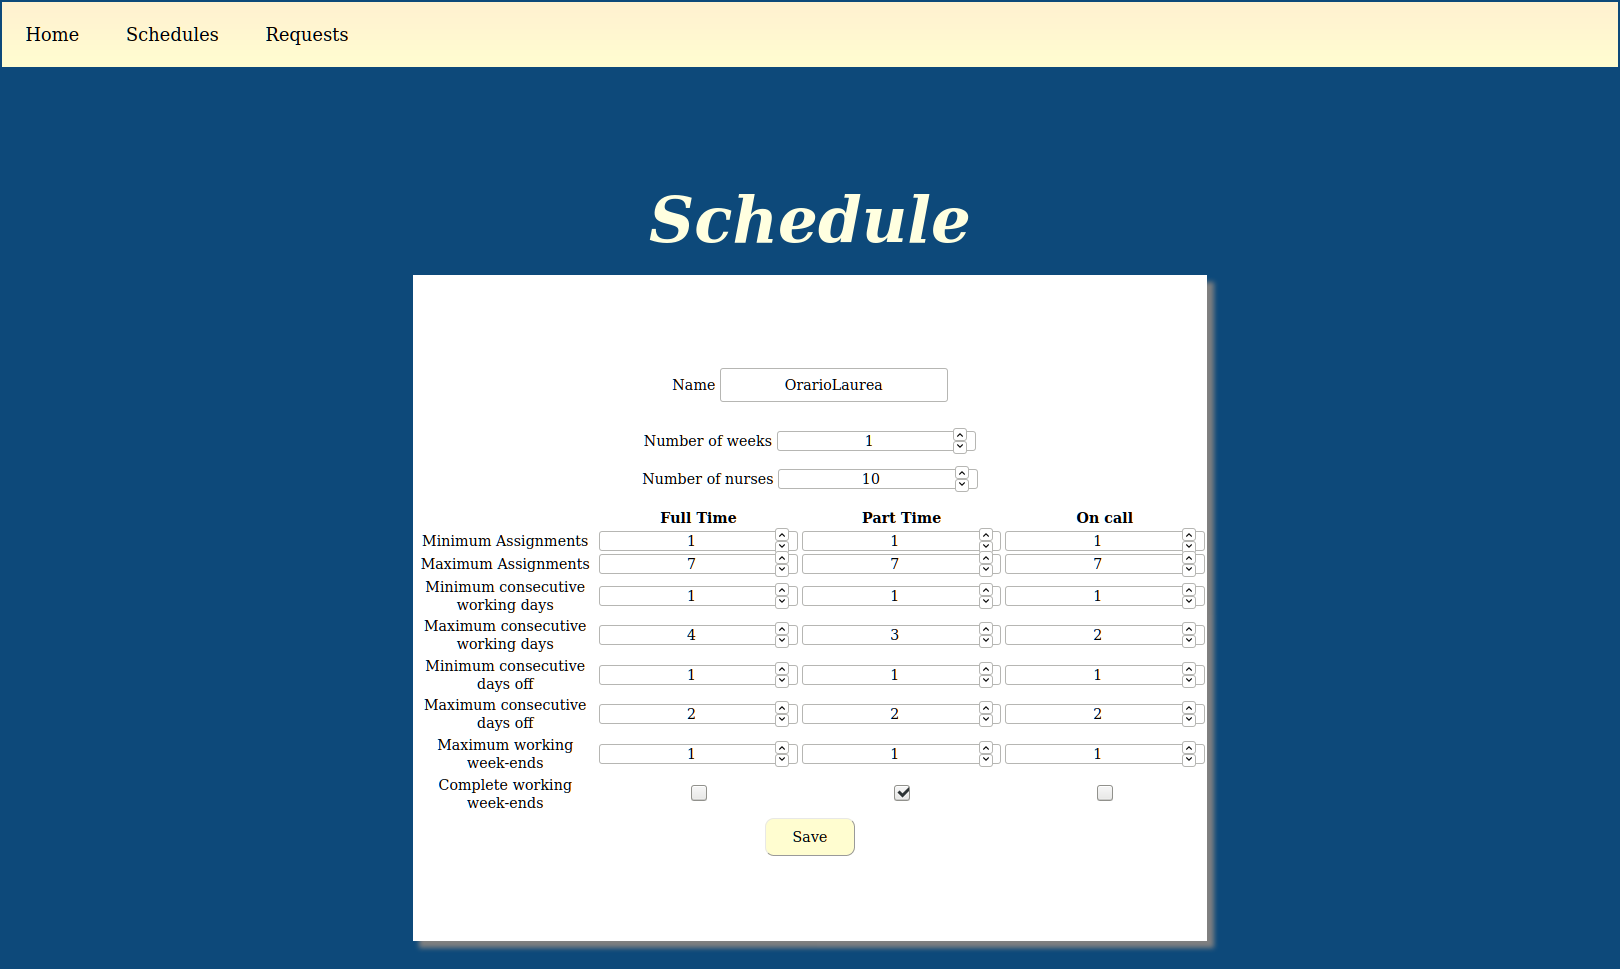
\includegraphics[width=\linewidth]{img/Schermate/S2.png}
\end{center}
\end{frame}

\begin{frame}
\frametitle{Interfaccia}
\begin{center}
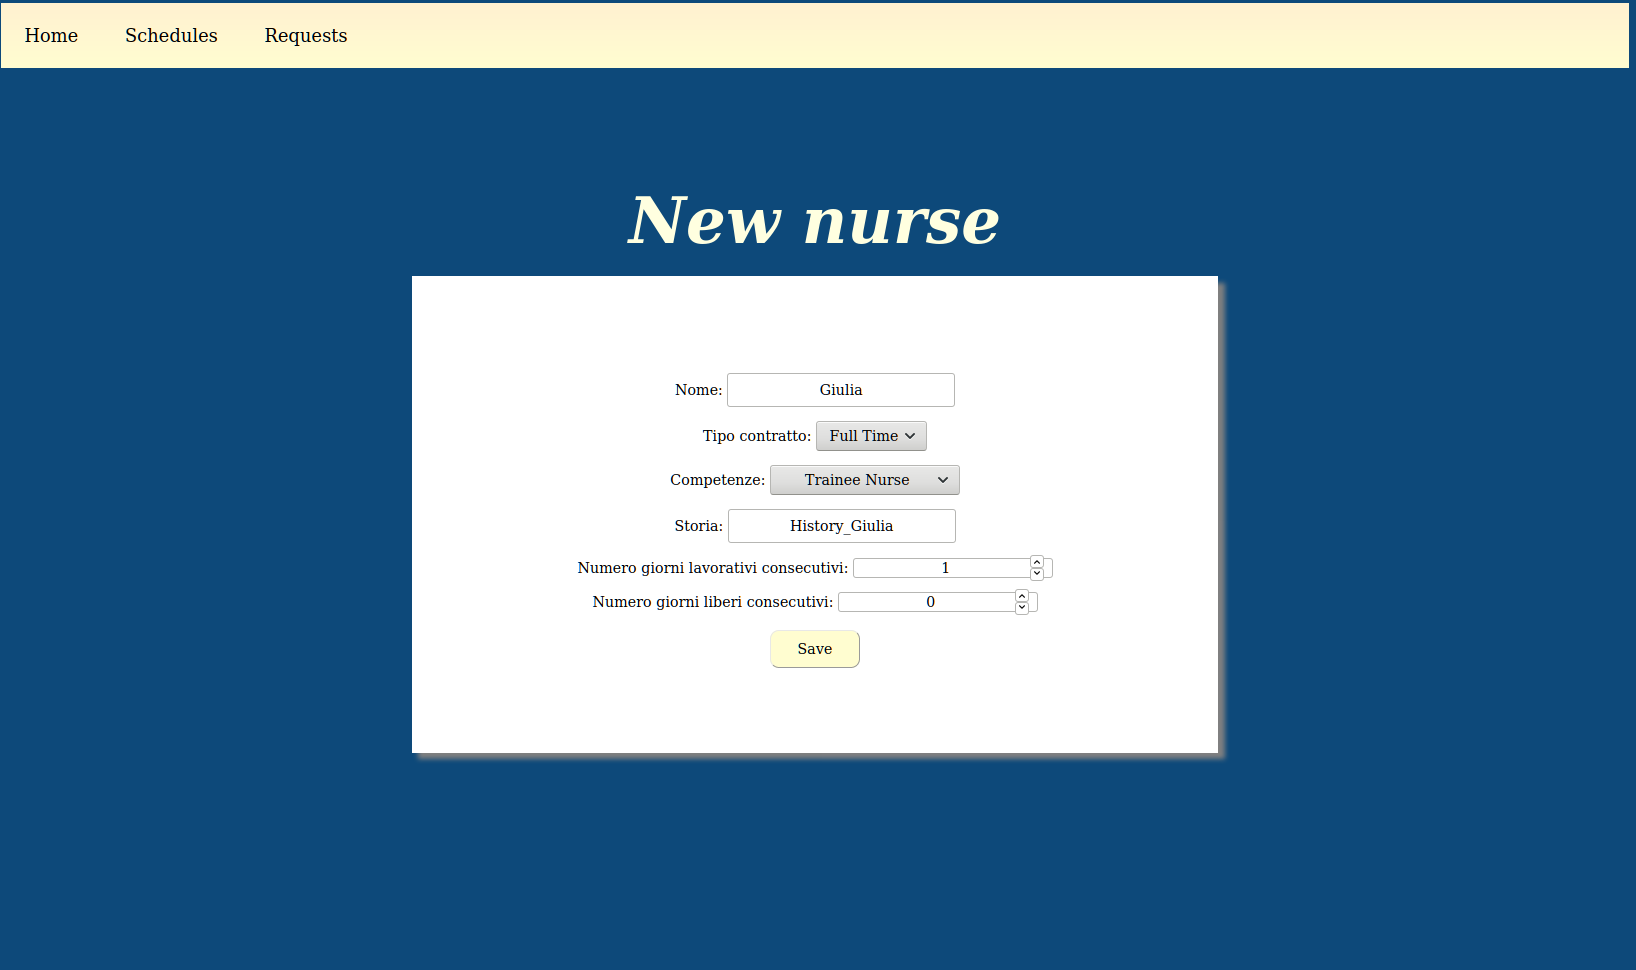
\includegraphics[width=\linewidth]{img/Schermate/S5.png}
\end{center}
\end{frame}

\begin{frame}
\frametitle{Interfaccia}
\begin{center}
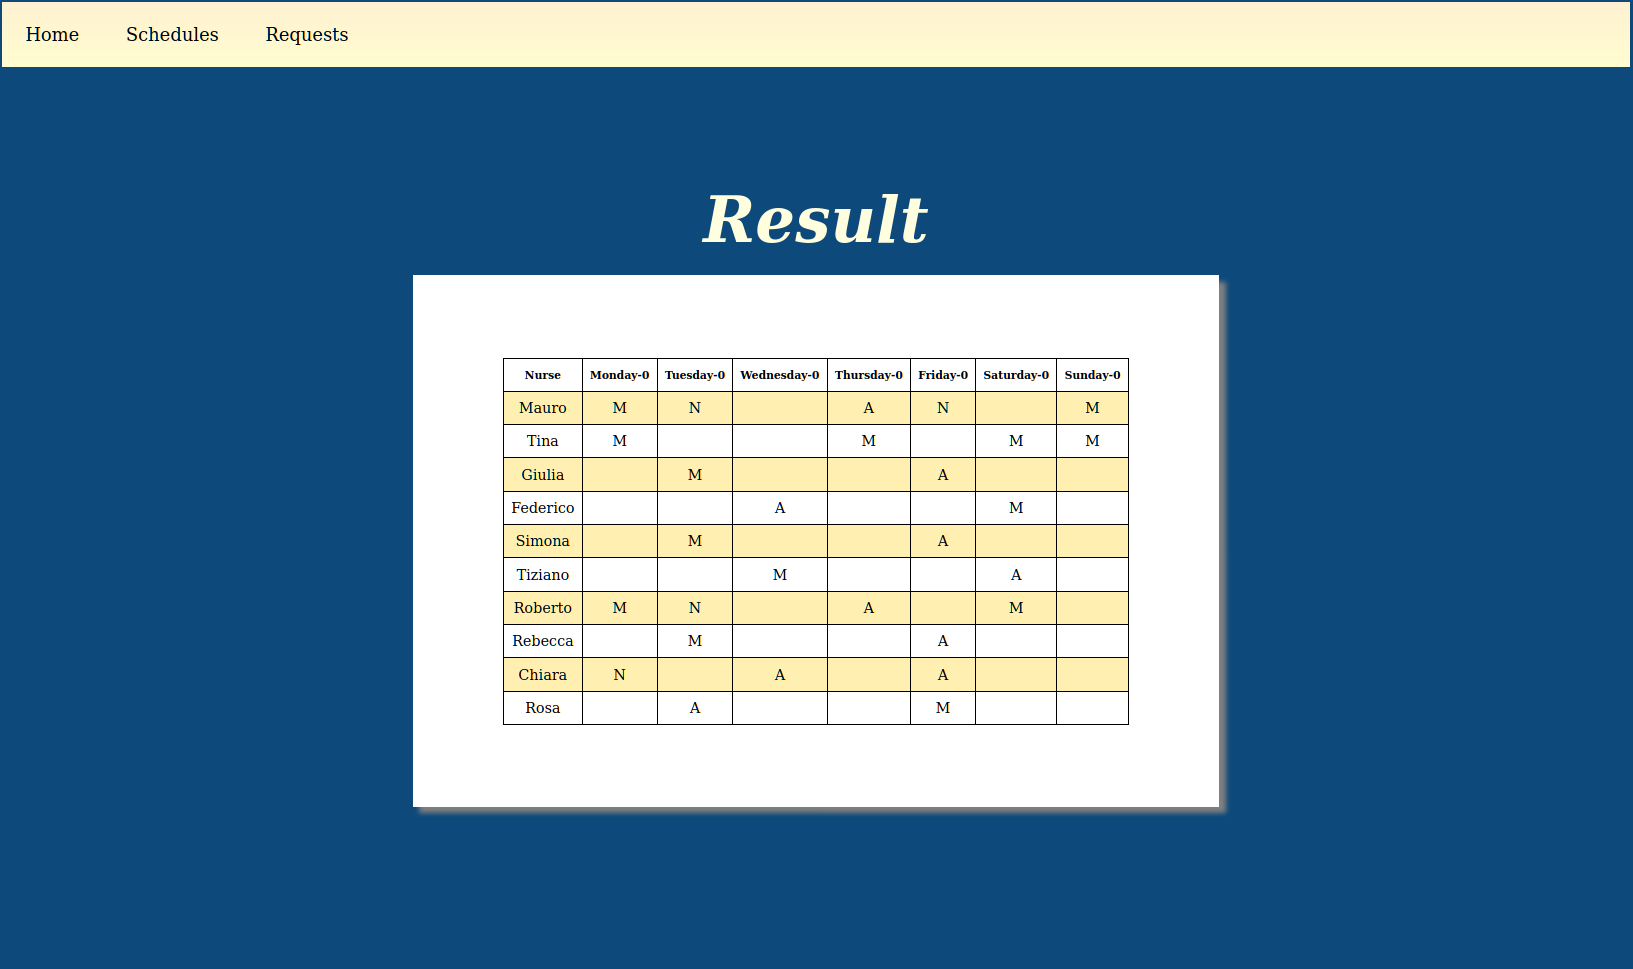
\includegraphics[width=\linewidth]{img/Schermate/Result.png}
\end{center}
\end{frame}

\begin{frame}
\frametitle{Tools}
\begin{columns}
\begin{column}{0.70\textwidth}
\begin{itemize}
\item Linguaggio di programmazione: \textit{Python}
\linebreak 
\linebreak
\item Software di ottimizzazione: \textit{Gurobi}
\linebreak 
\linebreak
\item Framework interfaccia: \textit{Django}
\end{itemize}
\end{column}
\begin{column}{0.40\textwidth}
\begin{figure}[h!]
	\begin{center}
  	\includegraphics[scale=0.02]{img/python2.png}
 	%\caption{}
	\end{center}
\end{figure}
\begin{figure}[h!]
	\begin{center}
  	\includegraphics[scale=0.2]{img/gurobi2.png}
 	%\caption{}
	\end{center}
\end{figure}

\begin{figure}[h!]
	\begin{center}
  	\includegraphics[scale=0.08]{img/LogoD.png}
 	%\caption{}
	\end{center}
\end{figure}
\end{column}
\end{columns}
\end{frame}


\begin{frame}
\frametitle{Fine}
Vi ringrazio per la vostra attenzione. Ci sono domande?
\end{frame}

%AGGIUNTIVI
\appendix

\begin{frame}[plain]
\end{frame}

\begin{frame}[noframenumbering]
\frametitle{Approfondimento Interfaccia}
\begin{center}
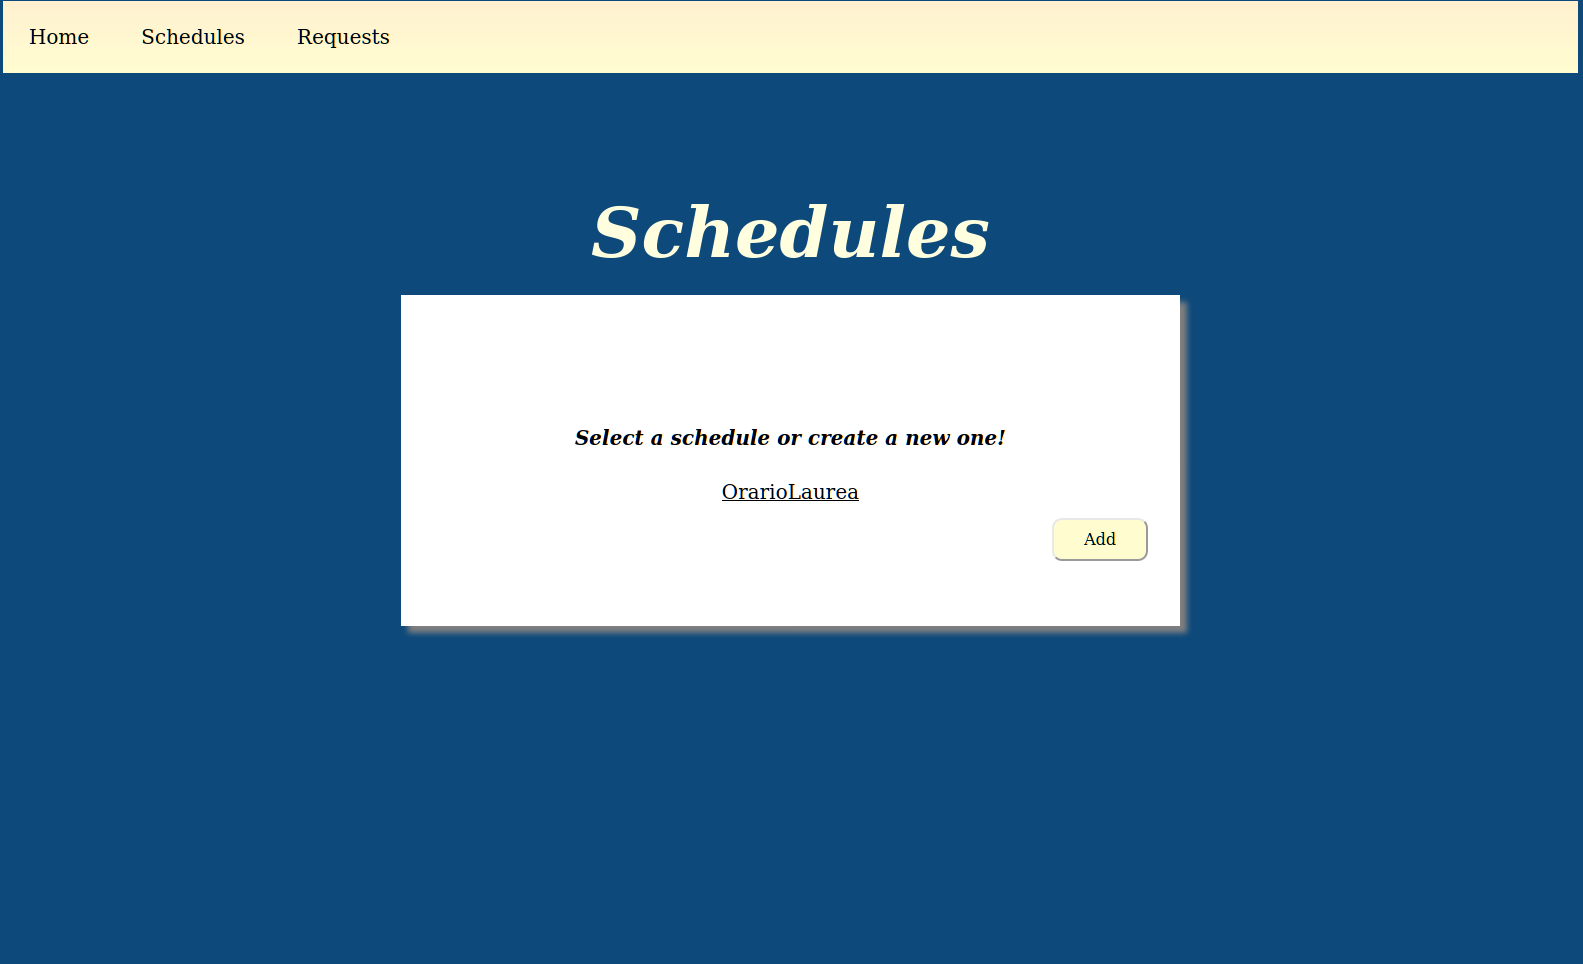
\includegraphics[width=\linewidth]{img/Schermate/S1.png}
\end{center}
\end{frame}

\begin{frame}[noframenumbering]
\frametitle{Approfondimento Interfaccia}
\begin{center}
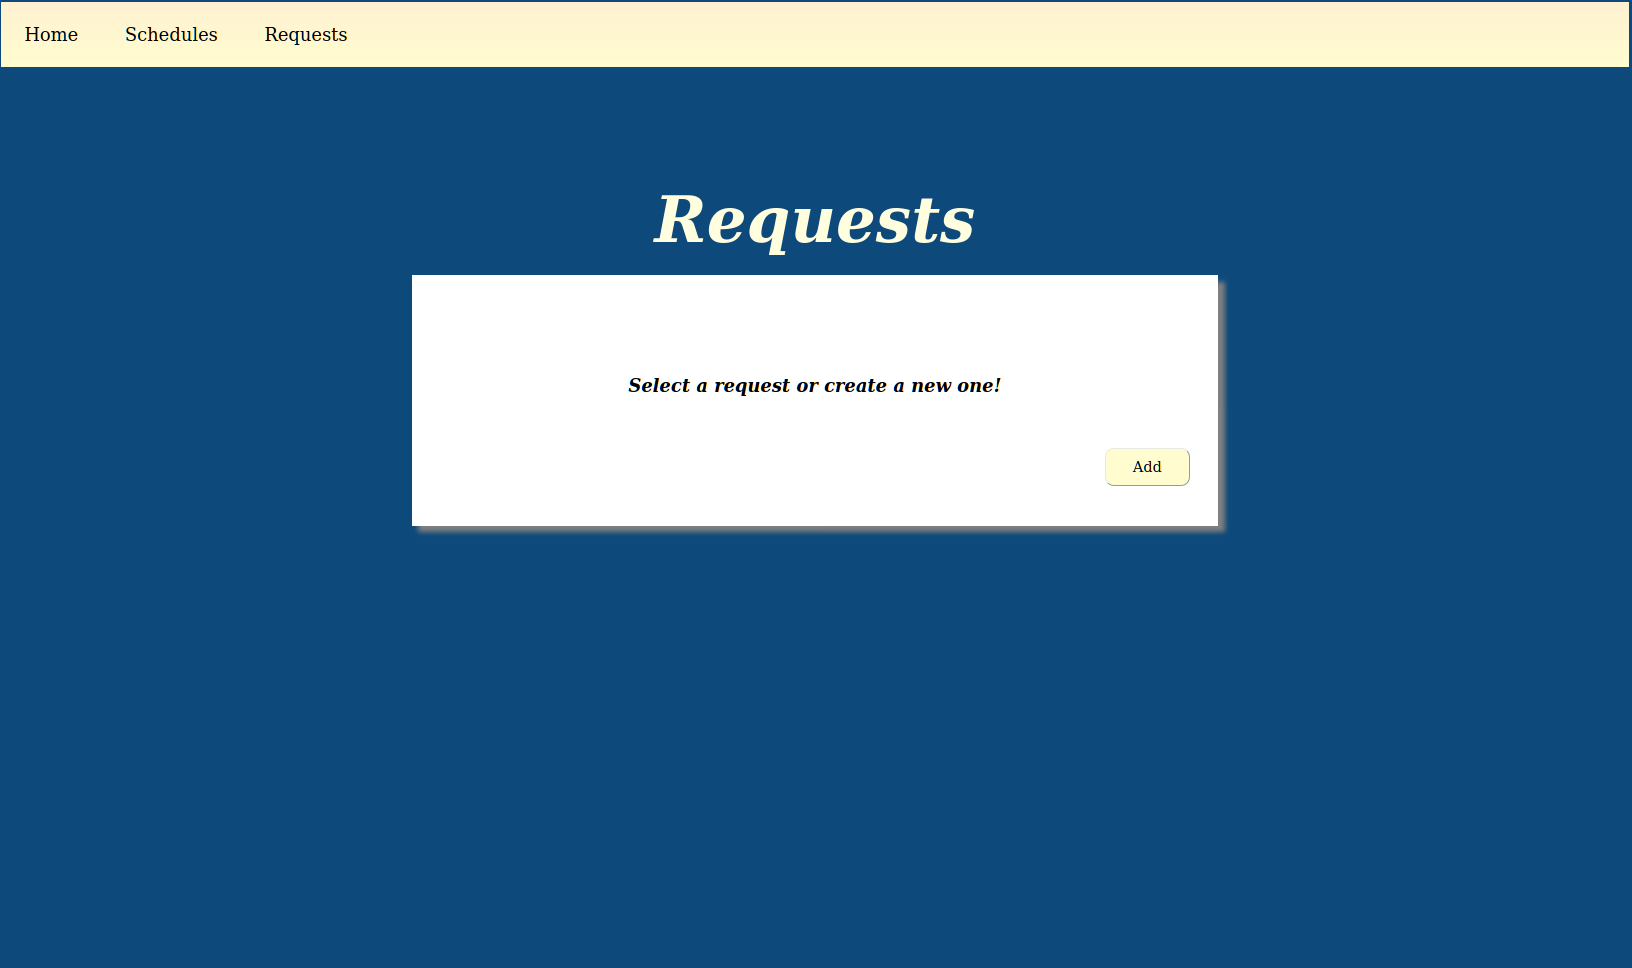
\includegraphics[width=\linewidth]{img/Schermate/S3.png}
\end{center}
\end{frame}

\begin{frame}[noframenumbering]
\frametitle{Approfondimento Interfaccia}
\begin{center}
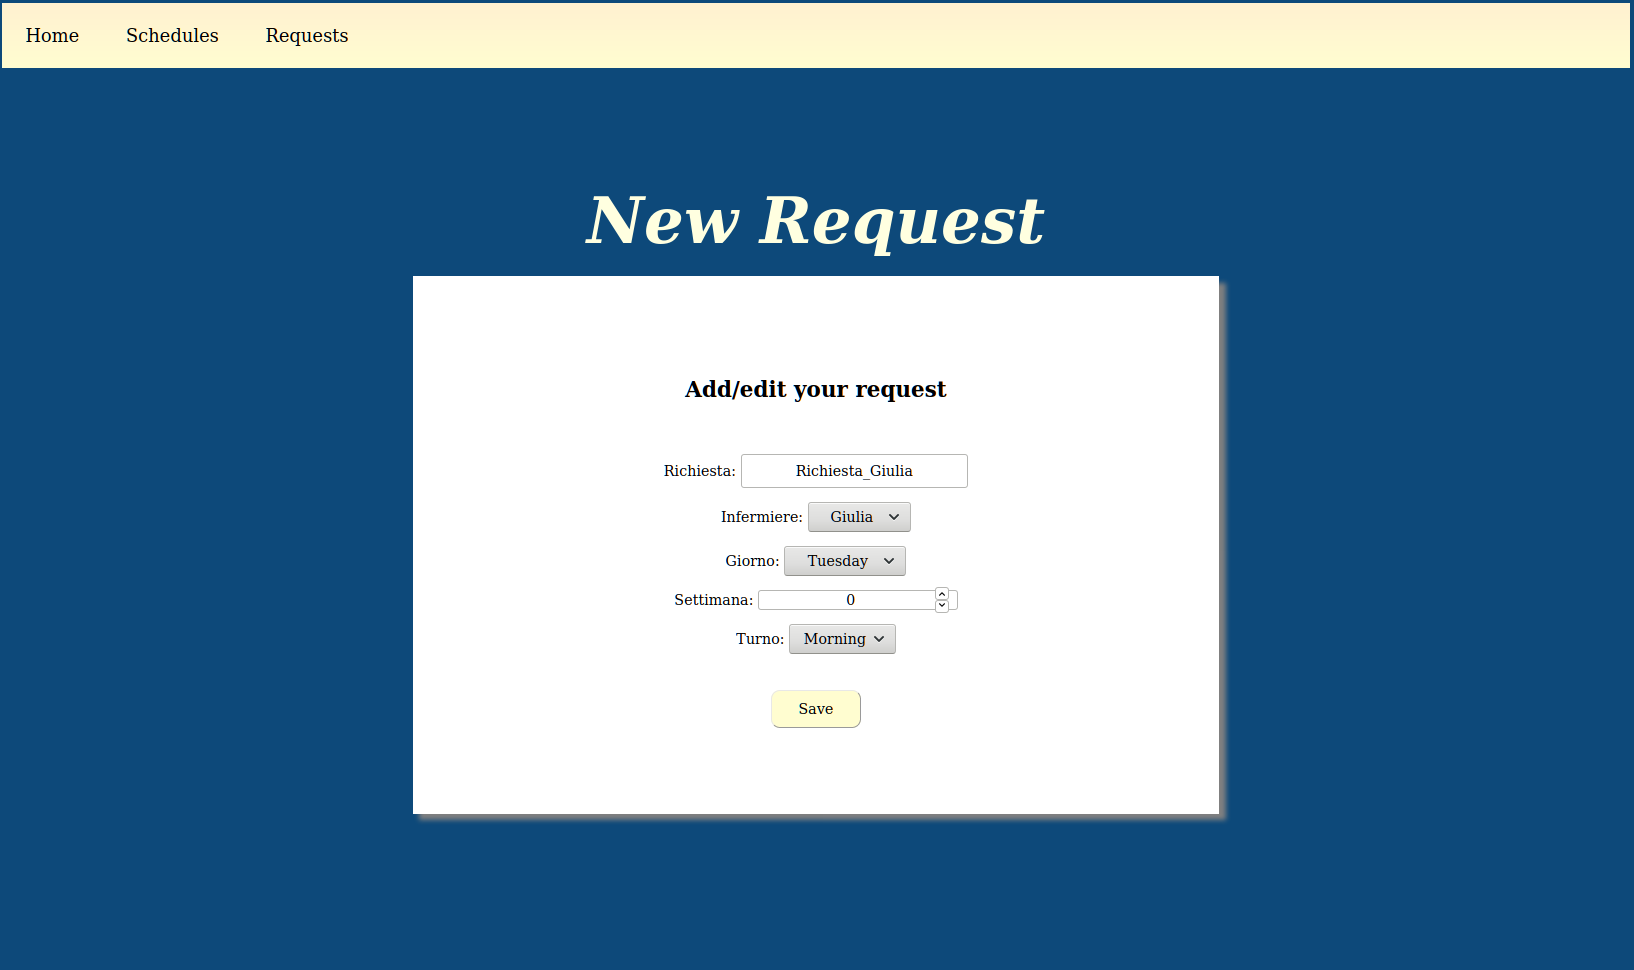
\includegraphics[width=\linewidth]{img/Schermate/S4.png}
\end{center}
\end{frame}

\begin{frame}[noframenumbering]
\frametitle{Approfondimento esperimenti}
Tempo di calcolo della soluzione con tempo massimo 1h
\begin{center}
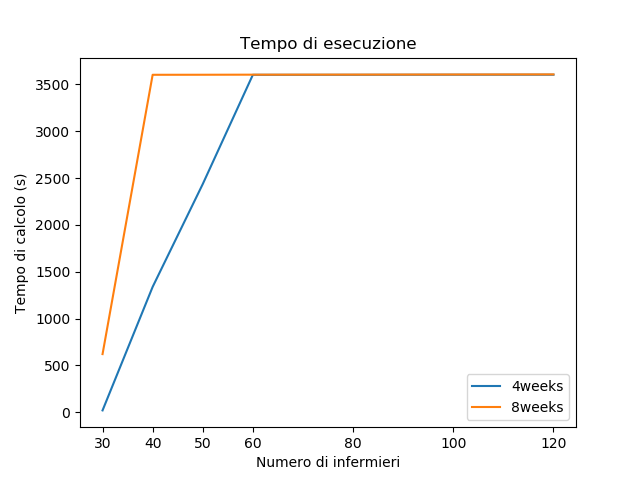
\includegraphics[scale=0.5]{img/Problema4/Time_1h-h1_w4.png}
\end{center}
\end{frame}

\begin{frame}[noframenumbering]
\frametitle{Approfondimento esperimenti}
Gap con tempo massimo 1h
\begin{center}
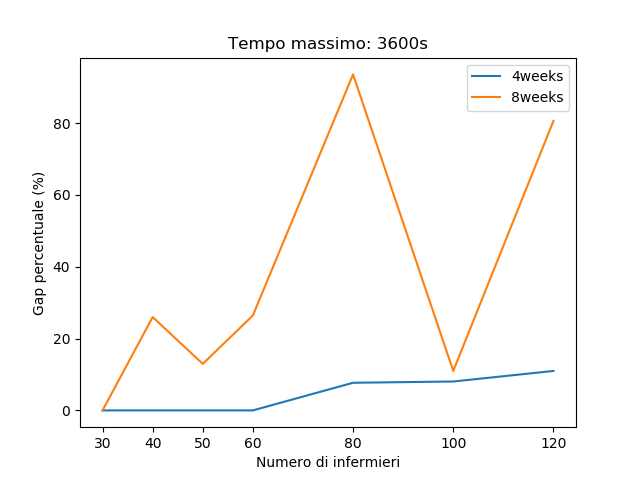
\includegraphics[scale=0.5]{img/Problema2/Gap_1h-h0_w4.png}
\end{center}
\end{frame}

\end{document}
